%\documentclass[compress,xcolor=table,9pt]{beamer}
\documentclass[xcolor=table,8pt]{beamer}

%%%%%%%%%%%%%%%%%%%%%%%%%%%%%%%%%%%%%%%%%%%%%%%%%%%%%%%%%%%%%%%%%%%%%%%%%%%%%%%%
% PACKAGES
%%%%%%%%%%%%%%%%%%%%%%%%%%%%%%%%%%%%%%%%%%%%%%%%%%%%%%%%%%%%%%%%%%%%%%%%%%%%%%%%
\usepackage{siunitx}
\usepackage{calc}
\usepackage{textpos}
\usepackage{physics}
\usepackage{amsmath}
\usepackage{amssymb}
\usepackage{tikz}
\usepackage{tikz-3dplot}
\usepackage{pgfplots}
\usepackage[compat=1.1.0]{tikz-feynman}
\usepackage{xparse}% So that we can have two optional parameters
\usepackage{mathtools}
\usepackage{eso-pic}
\usepackage{color,colortbl}
\usepackage{verbatim}
\usepackage{xmpmulti}
\usepackage{wrapfig}
\usepackage{booktabs} % Toprule, Midrule, Bottomrule
\usepackage[table]{xcolor} % Coloured tables
\usepackage{multicol} % Multicolumn cells
\usepackage{multirow} % Multirow cells
\usepackage{mdframed}
\usepackage{fancyhdr}
\usepackage{slashed}
\usepackage[htt]{hyphenat}
\usepackage{newunicodechar}
\usepackage{bold-extra}
\usepackage{appendixnumberbeamer}
\usepackage{graphbox}
\usepackage{tcolorbox}
\usepackage{todonotes}
\usepackage{subfig}
\usepackage{physics}
\usepackage{inconsolata}
\usepackage[mode=buildnew]{standalone}
\usepackage{pythonhighlight}
\usepackage[justification=justified]{caption}
\usepackage{transparent}
\usepackage{algpseudocode}
\usepackage{algorithm}
%%%%%%%%%%%%%%%%%%%%%%%%%%%%%%%%%%%%%%%%%%%%%%%%%%%%%%%%%%%%%%%%%%%%%%%%%%%%%%%%

\definecolor{linkcolor}{rgb}{0,0,0.65}
\definecolor{shadecolor}{rgb}{0.95, 0.95, 0.95}
\definecolor{mygreen}{rgb}{0,0.6,0}
\definecolor{myred}{rgb}{0.81, 0.06, 0.13}         %#CF1020
\definecolor{mygray}{rgb}{0.5,0.5,0.5}
\definecolor{mymauve}{rgb}{0.58,0,0.82}
\definecolor{mydmg}{rgb}{0.05, 0.5, 0.06}          %#00693E
\definecolor{blueinnerbox}{RGB}{229,230,238}
\definecolor{amber}{rgb}{1.0, 0.75, 0.0}
\definecolor{goldmetallic}{rgb}{0.83, 0.69, 0.22}
\definecolor{airforceblue}{rgb}{0.36, 0.54, 0.66}  %#5D8AA8
\definecolor{cobalt}{rgb}{0.0, 0.28, 0.67}         %#0047AB
\definecolor{coolblack}{rgb}{0.0, 0.18, 0.39}      %#002E63
\definecolor{dartmouthgreen}{rgb}{0.05, 0.5, 0.06} %#00693E
\definecolor{lava}{rgb}{0.81, 0.06, 0.13}          %#CF1020

\lstdefinestyle{python}
{
    backgroundcolor=\color{shadecolor},       % background color
    basicstyle=\ttfamily\footnotesize,        % the size of the fonts that are used for the code
    breakatwhitespace=false,                  % sets if automatic breaks should only happen at whitespace
    breaklines=true,                          % sets automatic line breaking
    postbreak=\mbox{\textcolor{black}{$\hookrightarrow$}\space},
    captionpos=b,                             % sets the caption-position to bottom
    commentstyle=\color{mygreen},             % comment style
    extendedchars=true,                       % lets you use non-ASCII characters; for 8-bits encodings only, does not work with UTF-8
    keepspaces=true,                          % keeps spaces in text, useful for keeping indentation of code (possibly needs columns=flexible)
    keywordstyle=\bfseries\color{blue},       % keyword style
    language=Python,                          % the language of the code
    numbers=left,                             % where to put the line-numbers; possible values are (none, left, right)
    numbersep=5pt,                            % how far the line-numbers are from the code
    numberstyle=\tiny\color{mygray},          % the style that is used for the line-numbers
    rulecolor=\color{black},                  % if not set, the frame-color may be changed on line-breaks within not-black text (e.g. comments (green here))
    showspaces=false,                         % show spaces everywhere adding particular underscores; it overrides 'showstringspaces'
    showstringspaces=false,                   % underline spaces within strings only
    showtabs=false,                           % show tabs within strings adding particular underscores
    stepnumber=1,                             % the step between two line-numbers. If it's 1, each line will be numbered
    stringstyle=\color{mymauve},              % string literal style
    tabsize=4,                                % sets default tabsize to 4 spaces
    title=\lstname                            % show the filename of files
}

\usepackage{pythonhighlight}



%%%%%%%%%%%%%%%%%%%%%%%%%%%%%%%%%%%%%%%%%%%%%%%%%%%%%%%%%%%%%%%%%%%%%%%%%%%%%%%%
% NEW COMMANDS
%%%%%%%%%%%%%%%%%%%%%%%%%%%%%%%%%%%%%%%%%%%%%%%%%%%%%%%%%%%%%%%%%%%%%%%%%%%%%%%%
%%% warning symbol
\newcommand\Warning{%
    \makebox[0.75em][c]{%
        \makebox[0pt][c]{\raisebox{.1em}{\small!}}%
        \makebox[0pt][c]{\color{red}\Large$\bigtriangleup$}%
    }%
}%
\newunicodechar{⚠}{\Warning}


%%% rvdots
\makeatletter
\DeclareRobustCommand{\rvdots}{%
    \vbox{
        \baselineskip4\p@\lineskiplimit\z@
        \kern-\p@
        \hbox{.}\hbox{.}\hbox{.}
    }}
\makeatother


%%% pgfplots
\newcommand\gauss[2]{1/(#2*sqrt(2*pi))*exp(-((x-#1)^2)/(2*#2^2))}


%%% colorboxes
\newcommand{\ok}[1]{ \colorbox{green!60!black}{\textcolor{white}{\textbf{#1}}} }
\newcommand{\kk}[1]{ \colorbox{orange}{\textcolor{white}{\textbf{#1}}} }
\newcommand{\ko}[1]{ \colorbox{red!80!black}{\textcolor{white}{\textbf{#1}}} }


%%% tikz rbox
\newcommand\RBox[2]{%
    \tikz\node[rounded corners,align=center,text width=#2] {#1};%
}
%%%%%%%%%%%%%%%%%%%%%%%%%%%%%%%%%%%%%%%%%%%%%%%%%%%%%%%%%%%%%%%%%%%%%%%%%%%%%%%%





%%%%%%%%%%%%%%%%%%%%%%%%%%%%%%%%%%%%%%%%%%%%%%%%%%%%%%%%%%%%%%%%%%%%%%%%%%%%%%%%
% SETTINGS
%%%%%%%%%%%%%%%%%%%%%%%%%%%%%%%%%%%%%%%%%%%%%%%%%%%%%%%%%%%%%%%%%%%%%%%%%%%%%%%%
%%% tikz libraries
\usetikzlibrary{calc,patterns,angles,quotes,arrows}
\usetikzlibrary{decorations,decorations.pathmorphing,decorations.markings,decorations.text}


%%% pgfplots
\pgfplotsset{compat=1.15,
    every axis/.append style={
        font=\large,
        line width=1pt,
        tick style={line width=0.8pt}
    }
}


%%% theme
\usetheme{Madrid}
% \usetheme{Szeged}
% \usetheme{Ilmenau}
\useoutertheme{noslidenum}


%%% theme color
\colorlet{beamer@blendedblue}{blue!40!black}


%%% theme font
%\usefonttheme[onlymath]{serif}
%\usefonttheme{serif}
%\setbeamerfont{title}{        family=\fontfamily{\sfdefault}\selectfont}
\setbeamerfont{frametitle}{   family=\fontfamily{\sfdefault}\selectfont\bfseries}
\setbeamerfont{framesubtitle}{family=\fontfamily{\sfdefault}\selectfont}
\setbeamerfont{title}{size=\huge}


%%% theme \pause configuration
\setbeamercovered{transparent}
%\setbeamercovered{dynamic}


%%% theme blocks style
\useinnertheme{rectangles}
% \setbeamertemplate{blocks}[rounded][shadow=false]
\setbeamertemplate{blocks}[default]
%\setbeamertemplate{title page}[custom][rounded=true]


%%% theme title page
\makeatletter
\defbeamertemplate*{title page}{custom}[1][rounded=true]
{
    \vbox{}
    \vfill
    \begingroup
        \centering
        {\usebeamercolor[fg]{titlegraphic}\inserttitlegraphic\par}
        \vskip2.0em
        \begin{beamercolorbox}[sep=6pt,center,#1]{title}
            \usebeamerfont{title}\inserttitle\par%
            \ifx\insertsubtitle\@empty%
            \else%
                \vskip0.25em%
                {\usebeamerfont{subtitle}\usebeamercolor[fg]{subtitle}\insertsubtitle\par}%
            \fi%
        \end{beamercolorbox}%
        \vskip2em\par
        \begin{beamercolorbox}[sep=6pt,center,#1]{author}
            \usebeamerfont{author}\insertauthor
        \end{beamercolorbox}
        \vskip1em\par
        \begin{beamercolorbox}[sep=6pt,center,#1]{institute}
            \usebeamerfont{institute}\insertinstitute
        \end{beamercolorbox}
        \begin{beamercolorbox}[sep=6pt,center,#1]{date}
            \usebeamerfont{date}\insertdate
        \end{beamercolorbox}
    \endgroup
    \vfill
}
\makeatother
%%%%%%%%%%%%%%%%%%%%%%%%%%%%%%%%%%%%%%%%%%%%%%%%%%%%%%%%%%%%%%%%%%%%%%%%%%%%%%%%





\title[\bfseries\fontfamily{\sfdefault}\selectfont TTN supervised classifier for HEP]{\fontfamily{\sfdefault}\selectfont\bfseries Tree Tensor Network supervised classifier\\for High Energy Physics}
% \subtitle{J.H. Hamilton, S. Hofmann, and Y.T. Oganessian}
\institute{\normalsize\bfseries\color{gray}Quantum Information and Computing\\a.y. 2020/21}
\titlegraphic{
	\includegraphics[height=2.0cm]{images/logos/unipd_logo.png}
}
% \author[R. Ardino and A. Valente]{\normalsize \begin{minipage}Rocco Ardino\\Mat. 1231629\end{minipage} \and Alessandro Valente\\Mat. 1234429}
\author[\bfseries\fontfamily{\sfdefault}\selectfont R. Ardino and A. Valente]
{%
   \texorpdfstring{
        \begin{columns}
            \column{.075\linewidth}
            \column{.425\linewidth}
            \centering
            \RBox{%
                \textbf{\normalsize \color{gray}Rocco Ardino}\\
                {\color{beamer@blendedblue}\footnotesize\bfseries {\fontfamily{\sfdefault}\selectfont Mat: 1231629}}\\
                \href{mailto:rocco.ardino@studenti.unipd.it}{\color{beamer@blendedblue}\texttt{\bfseries\footnotesize rocco.ardino@studenti.unipd.it}}%
            }{4.75cm}
            \column{.425\linewidth}
            \centering
            \RBox{%
                \textbf{\normalsize \color{gray}Alessandro Valente}\\
                {\color{beamer@blendedblue}\footnotesize\bfseries {\fontfamily{\sfdefault}\selectfont Mat: 1234429}}\\
                \href{mailto:alessandro.valente.4@studenti.unipd.it}{\color{beamer@blendedblue}\texttt{\bfseries\footnotesize alessandro.valente.4@studenti.unipd.it}}%
            }{4.75cm}
            \column{.075\linewidth}
        \end{columns}
   }
   {R. Ardino and A. Valente}
}
\date[\bfseries\fontfamily{\sfdefault}\selectfont March 19, 2021]{\small\bfseries \color{gray}March 19, 2021}





% remove when using \pause
\addtobeamertemplate{frametitle}{}{%
    \begin{textblock*}{110mm}(.885\textwidth,-0.775cm) %before -0.9cm
        \includegraphics[height=0.7cm]{images/logos/unipd_logo_white.png}
    \end{textblock*}
}


\beamertemplatenavigationsymbolsempty
% \addtobeamertemplate{navigation symbols}{}{%
%     \usebeamerfont{footline}%
%     \usebeamercolor[fg]{footline}%
%     \hspace{1em}%
%     \raisebox{1.5pt}[0pt][0pt]{\fontfamily{\sfdefault}\selectfont\color{blue}\textbf{\insertframenumber}/\textbf{\inserttotalframenumber}}
% }

\addtobeamertemplate{footline}{%
    \leavevmode%
    \hbox{%
        \begin{beamercolorbox}[
            wd=\paperwidth,
            ht=2.25ex,
            dp=1.0ex,
            center
        ]{author in head/foot}%
            \bfseries\fontfamily{\sfdefault}\selectfont\insertsectionnavigationhorizontal{\paperwidth}{}{}
        \end{beamercolorbox}
    }%
    \vspace{0.11pt}
}


\begin{document}

    %%%%%%%%%%%%%%%%%%%%%%%%%%%%%%%%%%%%%%%%%%%%%%%%%%%%%%%%%%%%%%%%%%%%%%%%%%%%
    % TITLE PAGE
    %%%%%%%%%%%%%%%%%%%%%%%%%%%%%%%%%%%%%%%%%%%%%%%%%%%%%%%%%%%%%%%%%%%%%%%%%%%%
    \begin{frame}[plain, noframenumbering]
        \titlepage
    \end{frame}
    %%%%%%%%%%%%%%%%%%%%%%%%%%%%%%%%%%%%%%%%%%%%%%%%%%%%%%%%%%%%%%%%%%%%%%%%%%%%

    %%%%%%%%%%%%%%%%%%%%%%%%%%%%%%%%%%%%%%%%%%%%%%%%%%%%%%%%%%%%%%%%%%%%%%%%%%%%
    % OUTLINE
    %%%%%%%%%%%%%%%%%%%%%%%%%%%%%%%%%%%%%%%%%%%%%%%%%%%%%%%%%%%%%%%%%%%%%%%%%%%%
    \begin{frame}[plain, noframenumbering]
        \frametitle{Outline}

        \tableofcontents
    \end{frame}
    %%%%%%%%%%%%%%%%%%%%%%%%%%%%%%%%%%%%%%%%%%%%%%%%%%%%%%%%%%%%%%%%%%%%%%%%%%%%



    \section{Introduction}

    %%%%%%%%%%%%%%%%%%%%%%%%%%%%%%%%%%%%%%%%%%%%%%%%%%%%%%%%%%%%%%%%%%%%%%%%%%%%
    % INTRODUCTION
    %%%%%%%%%%%%%%%%%%%%%%%%%%%%%%%%%%%%%%%%%%%%%%%%%%%%%%%%%%%%%%%%%%%%%%%%%%%%
    \begin{frame}[t]
        \frametitle{Introduction}
        
        \textbf{High Energy Physics (HEP)}:
        \begin{itemize}
            \item purpose of understanding the nature of the particles that constitute matter and radiation
            \item Standard Model as theoretical climax
            \item still lots of unanswered questions
            \item \( \Rightarrow \) \alert{still New Physics to discover}
        \end{itemize}
        
        \bigskip
        \textbf{Application of Machine Learning techniques in HEP}:
        \begin{itemize}
            \item current techniques used in HEP fail to capture all the available information
            \item as proved by Baldi et al ([\href{https://arxiv.org/pdf/1402.4735.pdf}{\alert{1}}]), Machine Learning can overcome this issue
            \item many other advantages, such as solution to the curse of high dimensionality of data
            \item e.g., Artificial Neural Networks exploited to build powerful classifiers
        \end{itemize}
        
        \bigskip
        New approach with \textbf{Tree Tensor Networks (TTN)}:
        \begin{itemize}
            \item \alert{quantum-inspired} version of Biological Neural Networks
            \item structure based on \alert{Tensor Network methods}
            \item possibility to solve non-convex optimisation tasks, such as loss functions minimisation
        \end{itemize}
    \end{frame}
    %%%%%%%%%%%%%%%%%%%%%%%%%%%%%%%%%%%%%%%%%%%%%%%%%%%%%%%%%%%%%%%%%%%%%%%%%%%%





    \section{Theory}
    
    \subsection{Kinematics of high energy collisions}
    %%%%%%%%%%%%%%%%%%%%%%%%%%%%%%%%%%%%%%%%%%%%%%%%%%%%%%%%%%%%%%%%%%%%%%%%%%%%
    % THEORY::KINEMATICS
    %%%%%%%%%%%%%%%%%%%%%%%%%%%%%%%%%%%%%%%%%%%%%%%%%%%%%%%%%%%%%%%%%%%%%%%%%%%%
    \begin{frame}[t]
        \frametitle{Kinematics of high energy collisions}
        
        \begin{figure}[!h]
            \begin{minipage}[c]{0.50\linewidth}
                \vspace{0pt}
                \centering
                \subfloat[Kinematics of a collision]{
                    \includestandalone[mode=tex, height=3.5cm]{images/theory/lhc}
                    \label{fig:theory_kinematics_map}
                }
            \end{minipage}%
            \begin{minipage}[c]{0.50\linewidth}
                \vspace{0pt}
                \centering
                \subfloat[Pseudorapidity visualisation]{
                    \includestandalone[mode=tex, height=3.5cm]{images/theory/eta}
                    \label{fig:theory_kinematics_eta}
                }
            \end{minipage}%
            \caption{LHC structure and kinematics of a product particle, emitted with a polar angle \( \theta \) and azimuth angle \( \phi \), in \textbf{\ref{fig:theory_kinematics_map}}. In \textbf{\ref{fig:theory_kinematics_eta}}, visualisation of the linking between the polar angle and the pseudorapidity \( \eta \).}
            \label{fig:theory_kinematics_map_eta}
        \end{figure}

        \newcommand\brabarb{\scalebox{.3}{(}\raisebox{-1.7pt}[0pt][0pt]{$-$}\scalebox{.3}{)}}
        \vspace{-20pt}
        \begin{columns}
            \column[T]{0.475\textwidth}
            \begin{center}
                \begin{block}{Product particles of \( pp \) collisions}
                    \begin{itemize}
                        \item Leptons (\( \ell^{\pm} \), \( \overset{\brabarb}{\nu_{\ell}} \)) 
                        \item Bosons (\( h^{0} \), \( Z^{0} \), \( W^{\pm} \))
                        \item Quarks (\( q \)) and Gluons (\( g \))
                        \item Jets from quark/gluon hadronisation (\( j \))
                    \end{itemize}
                \end{block}
            \end{center}
            \column[T]{0.475\textwidth}
            \begin{center}
                \begin{block}{Main features for the analysis}
                    \begin{itemize}
                        \item Transverse momentum \( p_{\text{T}} \)
                        \item Pseudorapidity \( \eta \)
                        \item Azimuth angle \( \phi \)
                        \item \( b \)-tag (for jets)
                    \end{itemize}
                \end{block}
            \end{center}
        \end{columns}
    \end{frame}
    %%%%%%%%%%%%%%%%%%%%%%%%%%%%%%%%%%%%%%%%%%%%%%%%%%%%%%%%%%%%%%%%%%%%%%%%%%%%



    \subsection{HIGGS dataset}
    %%%%%%%%%%%%%%%%%%%%%%%%%%%%%%%%%%%%%%%%%%%%%%%%%%%%%%%%%%%%%%%%%%%%%%%%%%%%
    % THEORY::HIGGS
    %%%%%%%%%%%%%%%%%%%%%%%%%%%%%%%%%%%%%%%%%%%%%%%%%%%%%%%%%%%%%%%%%%%%%%%%%%%%
    \begin{frame}[t]
        \frametitle{HIGGS dataset}
        
        \textbf{Monte Carlo generated sample of gluon fusion process}:
        \begin{itemize}
            \item a mass of the Higgs \( m_{h^{0}} = 125 \ \si{GeV} \) is assumed
            \item \alert{new exotic Higgs bosons \( H^{0} \) and \( H^{\pm} \)} are introduced (\( m_{H^{0}} = 425 \ \si{GeV} \), \( m_{H^{\pm}} = 325 \ \si{GeV} \))
            \item \alert{21 low level features} (such as \( p_{\text{T}} \), \( \eta \), \( \phi \), \( b \)-tags, \dots)
            \item \alert{7 high level features} (invariant masses distributions)
        \end{itemize}
        
        \begin{figure}[!h]
            \begin{minipage}[c]{0.50\linewidth}
                \vspace{0pt}
                \centering
                \subfloat[Signal process]{
                    \includestandalone[mode=tex, height=3.0cm]{images/theory/signal}
                    \label{fig:theory_HIGGS_signal}
                }
            \end{minipage}%
            \begin{minipage}[c]{0.50\linewidth}
                \vspace{0pt}
                \centering
                \subfloat[Background process]{
                    \includestandalone[mode=tex, height=3.0cm]{images/theory/background}
                    \label{fig:theory_HIGGS_background}
                }
            \end{minipage}%
            \caption{Feynman diagrams for the Monte Carlo simulated events. In \textbf{\ref{fig:theory_HIGGS_signal}}, the diagram of the signal channel is portrayed with the exotic Higgs bosons \( H^{0} \) and \( H^{\pm} \). In \textbf{\ref{fig:theory_HIGGS_background}}, the background diagram is represented.}
            \label{fig:theory_HIGGS_feynman}
        \end{figure}
        
        \vspace{-20pt}
        \begin{align}
            \text{\bfseries Signal:} \qquad&\alert{gg} \to
                H^{0}
                \to
                W^{\mp} H^{\pm}
                \to
                W^{\mp} W^{\pm} h^{0}
                \to
                \alert{W^{\mp} W^{\pm} b \bar{b}}
                \\
            \text{\bfseries Background:} \qquad&\alert{gg} \to
                g
                \to
                t \bar{t}
                \to
                \alert{W^{\mp} W^{\pm} b \bar{b}}
        \end{align}
    \end{frame}
    %%%%%%%%%%%%%%%%%%%%%%%%%%%%%%%%%%%%%%%%%%%%%%%%%%%%%%%%%%%%%%%%%%%%%%%%%%%%
    
    
    
    \subsection{Tree Tensor Networks}
    %%%%%%%%%%%%%%%%%%%%%%%%%%%%%%%%%%%%%%%%%%%%%%%%%%%%%%%%%%%%%%%%%%%%%%%%%%%%
    % THEORY::TTN
    %%%%%%%%%%%%%%%%%%%%%%%%%%%%%%%%%%%%%%%%%%%%%%%%%%%%%%%%%%%%%%%%%%%%%%%%%%%%
    \begin{frame}[t]
        \frametitle{Tensor Networks}
        
        \textbf{Tensor Networks (TNs) as core of TTNs}:
        \begin{itemize}
            \item \alert{factorisations of high rank tensors into networks of smaller rank tensors}
            \item intuitive graphical language
            \begin{itemize}
                \item tensors are notated by solid shapes, tensor indices are notated by lines emanating from these shapes
                \item connecting two index lines implies a contraction, or summation over the connected indices
                \begin{equation}
                    \begin{array}{ c @{\extracolsep{0.25cm}} c c c @{\extracolsep{0.25cm}} c }
                        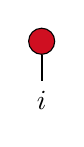
\begin{tikzpicture}[baseline={([yshift=-.5ex]current bounding box.center)}]
                            \node[draw, shape=circle, fill=lava] (n0) at (0,0)  {};
                            \node                     (i0) at (0,-0.75) {\( i \)};
                            \draw [thick] (n0) -- (i0);
                        \end{tikzpicture}
                        &=& v_{i} &\longrightarrow&   \textbf{Vector}
                        \\
                        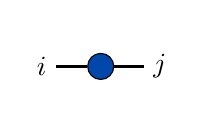
\begin{tikzpicture}[baseline={([yshift=-.5ex]current bounding box.center)}]
                            \node[draw, shape=circle, fill=cobalt] (n0) at (0,0)  {};
                            \node                     (i0) at (-0.75,0) {\( i \)};
                            \node                     (i1) at ( 0.75,0) {\( j \)};
                            \node                     (e0) at ( 0   ,-0.375) {~};
                            \node                     (e1) at ( 0   , 0.375) {~};
                            \draw [thick] (i0) -- (n0);
                            \draw [thick] (i1) -- (n0);
                        \end{tikzpicture}
                        &=&   M_{ij}  &\longrightarrow&   \textbf{Matrix}
                        \\
                        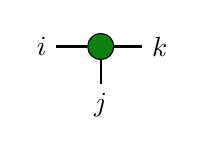
\begin{tikzpicture}[baseline={([yshift=-.5ex]current bounding box.center)}]
                            \node[draw, shape=circle, fill=dartmouthgreen] (n0) at (0,0)  {};
                            \node                     (i0) at (-0.75, 0   ) {\( i \)};
                            \node                     (i1) at ( 0   ,-0.75) {\( j \)};
                            \node                     (i2) at ( 0.75, 0   ) {\( k \)};
                            \draw [thick] (i0) -- (n0);
                            \draw [thick] (i1) -- (n0);
                            \draw [thick] (i2) -- (n0);
                        \end{tikzpicture}
                        &=&   T_{ijk} &\longrightarrow&   \textbf{Rank-3 Tensor}
                    \end{array}
                \end{equation}
            
                \item graphical notation for some of the most common operations between tensors
                \begin{equation}
                    \begin{array}{ l @{\extracolsep{0.25cm}} c c c @{\extracolsep{0.25cm}} c }
                        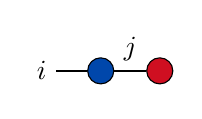
\begin{tikzpicture}[baseline={([yshift=-.5ex]current bounding box.center)}]
                            \node[draw, shape=circle, fill=cobalt] (n0) at (0,0)  {};
                            \node[draw, shape=circle, fill=lava]   (n1) at (0.75,0)  {};
                            \node                                  (i0) at (-0.75,0) {\( i \)};
                            \draw [thick] (i0) -- (n0);
                            \draw [thick] (n0) -- (n1) node[midway,anchor=south] {\( j \)}     node[midway,anchor=north] {~};;
                        \end{tikzpicture}
                        &=&   {\displaystyle\sum_{j} M_{ij}v_{j}} &\longrightarrow&       \textbf{Vector-Matrix}
                        \\
                        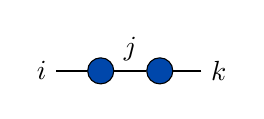
\begin{tikzpicture}[baseline={([yshift=-.5ex]current bounding box.center)}]
                            \node[draw, shape=circle, fill=cobalt] (n0) at (0,0)  {};
                            \node[draw, shape=circle, fill=cobalt] (n1) at (0.75,0)  {};
                            \node                                  (i0) at (-0.75,0) {\( i \)};
                            \node                                  (i1) at ( 1.50,0) {\( k \)};
                            \draw [thick] (i0) -- (n0);
                            \draw [thick] (i1) -- (n1);
                            \draw [thick] (n0) -- (n1) node[midway,anchor=south] {\( j \)}     node[midway,anchor=north] {~};
                        \end{tikzpicture}
                        &=&   {\displaystyle\sum_{j} A_{ij}B_{jk}}    &\longrightarrow&       \textbf{Matrix-Matrix}
                    \end{array}
                \end{equation}
            \end{itemize}
        \end{itemize}
    \end{frame}
    
    
    \begin{frame}[t]
        \frametitle{Tree Tensor Networks}
        
        \textbf{TNs for Machine Learning in a nutshell}:
        \begin{itemize}
            % \item definition using the formalism of Quantum Mechanics:
            \item input features \( x \), mapped into \( \Phi(x) \) through an apposite feature map
            \item TN with a tree-like structure \( T(w;\chi) \), with:
            \begin{itemize}
                \item \textbf{\( \boldsymbol{w} \) the entries of the tensors}, namely the weights to be tuned by the learning algorithm
                \item \textbf{\( \alert{\boldsymbol{\chi}} \) the bond dimension}, which controls the complexity of the structure
            \end{itemize}
            \item decision function: \alert{\( f(x;w) = T(w;\chi) \cdot \Phi(x) \)}
        \end{itemize}

        \begin{figure}[!h]
            \begin{minipage}[c]{0.50\linewidth}
                \vspace{0pt}
                \centering
                \subfloat[Example of TTN structure]{
                    \includestandalone[mode=tex, height=4.0cm]{images/theory/TTN}
                    \label{fig:theory_TTN_TTN_structure}
                }
            \end{minipage}%
            \begin{minipage}[c]{0.50\linewidth}
                \vspace{0pt}
                \centering
                \subfloat[Example of DNN structure]{
                    \includestandalone[mode=tex, height=4.0cm]{images/theory/DNN}
                    \label{fig:theory_TTN_DNN_structure}
                }
            \end{minipage}%
            \caption{Comparison between examples of structures for a TTN, in \textbf{\ref{fig:theory_TTN_TTN_structure}}, and a DNN, in \textbf{\ref{fig:theory_TTN_DNN_structure}}. In particular, in the TTN the dimension of the bonds between the tensors in the hidden layers is the bond dimension \( \chi \).}
            \label{fig:theory_TTN_TTN_DNN_structures}
        \end{figure}
    \end{frame}
    
    
    \begin{frame}[t]
        \frametitle{TTN Learning algorithm}
        
        \textbf{Loss function}:
        \begin{itemize}
            \item need to minimise the ladder on a fraction of dataset reserved for training the TTN
            \item quantification of TTN misclassification on new fraction of dataset reserved for validation
            \item \alert{binary cross-entropy} possible loss for signal-versus-background discrimination with:
            \begin{itemize}
                \item \( y_{\text{true}}^{(i)} \): true label of \( i^{\text{th}} \) sample of validation set
                \item \( y_{\text{pred}}^{(i)} \): TTN predicted label for the \( i^{\text{th}} \) sample of validation set
            \end{itemize}
            \begin{equation}
                L(y_{\text{true}}, y_{\text{pred}})
                =
                \sum_{i}^{n_{\text{val}}}
                y_{\text{true}}^{(i)} \log\qty(y_{\text{pred}}^{(i)}) + (1-y_{\text{true}}^{(i)}) \log\qty(1 - y_{\text{pred}}^{(i)})
            \end{equation}
        \end{itemize}
        
        \medskip
        \textbf{Metrics for performances quantification}:
        \begin{itemize}
            \item \alert{accuracy}: fraction of correctly classified samples (using a decision threshold \( \xi \in (0,1) \))
            \item \alert{AUC}: area under the Receiver Operating Characteristic (ROC) Curve
            \begin{itemize}
                \item True Positive Rate (TPR) in function of the False Positive Rate (FPR)
                \item obtained by sweeping the decision threshold \( \xi \) in \( (0,1) \)
                \item directly linked to concept of discovery significance commonly used in HEP
            \end{itemize}
        \end{itemize}
        
        \medskip
        \textbf{Optimiser for weights update}:
        \begin{itemize}
            \item \alert{ADAM}: adapts the correction to the weights at each step parameter per parameter
            \item update after the TTN has processed a \alert{mini batch} of input training set of dimension \( m \)
            \item after processing all mini batches in the training set, a \alert{training epoch} has ended
        \end{itemize}
    \end{frame}
    %%%%%%%%%%%%%%%%%%%%%%%%%%%%%%%%%%%%%%%%%%%%%%%%%%%%%%%%%%%%%%%%%%%%%%%%%%%%
    
    
    
    \subsection{Advanced techniques}
    %%%%%%%%%%%%%%%%%%%%%%%%%%%%%%%%%%%%%%%%%%%%%%%%%%%%%%%%%%%%%%%%%%%%%%%%%%%%
    % THEORY::ADVANCED
    %%%%%%%%%%%%%%%%%%%%%%%%%%%%%%%%%%%%%%%%%%%%%%%%%%%%%%%%%%%%%%%%%%%%%%%%%%%%
    \begin{frame}[t]
        \frametitle{Advanced techniques for performance boosting}
        
        \textbf{Activation function}:
        \begin{itemize}
            \item function applied at the output of a layer
            \item source of non-linearity to enlarge the space of functions that the TTN can approximate
            \item for this work, \alert{ELU} (for inner layers) and \alert{sigmoid} (for output layer) tested:
        \end{itemize}
        \begin{equation}
            \text{ELU}(x)
            =
            \begin{cases}
                x   &   x \ge 0 \\
                a(e^{x}-1)  &   x < 0
            \end{cases}
            \qquad\qquad
            \sigma(x)
            =
            \frac{1}{1 + e^{-x}}
        \end{equation}
        
        \medskip
        \textbf{Kernel regularisation}:
        \begin{itemize}
            \item add a penalty for large weights to the loss function to avoid overfit
            \item \alert{\( \ell_{2} \) regularisation}:
        \end{itemize}
        \begin{equation}
            J(y_{\text{true}}, y_{\text{pred}})
            =
            L(y_{\text{true}}, y_{\text{pred}})
            +
            \lambda \sum_{i=1}^{n_{\text{weights}}} \abs{w_{i}}^{2}
        \end{equation}
        
        \medskip
        \textbf{Batch normalisation}:
        \begin{itemize}
            \item training networks with lots of layer is very challenging
            \item calculate mean and standard deviation of the output of each layer for every mini batch
            \item \( \Rightarrow \) perform a \alert{standardisation}
            \item \( \Rightarrow \) \alert{speed up of learning algorithm convergence}
        \end{itemize}
    \end{frame}
    %%%%%%%%%%%%%%%%%%%%%%%%%%%%%%%%%%%%%%%%%%%%%%%%%%%%%%%%%%%%%%%%%%%%%%%%%%%%
    
    
    







    \section{Code Implementation}

    \subsection{Input data preprocessing}
    %%%%%%%%%%%%%%%%%%%%%%%%%%%%%%%%%%%%%%%%%%%%%%%%%%%%%%%%%%%%%%%%%%%%%%%%%%%%
    % CODE::PREPROCESSING
    %%%%%%%%%%%%%%%%%%%%%%%%%%%%%%%%%%%%%%%%%%%%%%%%%%%%%%%%%%%%%%%%%%%%%%%%%%%%
    \begin{frame}[t]
        \frametitle{Input data preprocessing}

        \textbf{Input features preprocessing workflow}:
        \begin{itemize}
            \item \alert{rescaled} in \( [0,1] \) or \( [-1,1] \) (depending on the feature)
            \item \alert{padded} to match the number of input ``legs'' of the TTN
            \item \alert{mapped} through a feature map to enhance the performances
        \end{itemize}

        \vspace{5pt}
        \begin{figure}[!h]
            \centering
            \includestandalone[mode=tex, width=0.70\textwidth]{images/code/workflow}
            \caption{Workflow of preprocessing precedure, starting from the rescaling of data, going through the zero padding in order to get proper dimensions for the input of the TTN, and lastly the polynomial or spherical mapping.}
            \label{fig:code_preprocessing_workflow}
        \end{figure}
    \end{frame}
    
    
    \begin{frame}[t,fragile]
        \frametitle{Input data preprocessing: rescaling and padding}
        % \vspace{-3mm}
        
        \textbf{Rescaling}
        \begin{itemize}
            \item rescale ``positive'' and ``negative'' features in \( [0,1] \) and \( [-1,1] \), respectively
        \end{itemize}

        \begin{equation}
            \alert{
                x^{(i)}_{j}
                \longrightarrow
                x^{(i)\prime}_{j}
                =
                \frac{x^{(i)}_{j}}{m_j}
            }
            \quad \text{with} \quad
            m_{j}
            =
            \max_{i\in \mathcal{D}_{\mathrm{train}}} \abs{x^{(i)}_{j}}
        \end{equation}
        
        % \smallskip
        \textbf{Padding}
        \begin{itemize}
            \item total number of features \( n_{\text{f}} \) must be divisible by features contracted in each site \( n_{\text{con}} \)
            \item dataset is ``padded'' with fictitious features to reach \( \tilde{n}_{\text{f}} \) features
        \end{itemize}
        
        \begin{equation}
            \alert{
                \tilde{n}_{\text{f}}
                =
                \min_{n\in\mathbb{N}}
                \qty{n \ge n_{\text{f}} \ : \ n = \qty(n_{\text{con}})^{m} \ , \ m \in \mathbb{N} }
            }
        \end{equation}
        
        % \begin{lstlisting}[    style=mypython, frame=single,    aboveskip=10pt, belowskip=10pt]
        % \vspace{-5pt}
        \begin{lstlisting}[style=mypython, numbers=none, frame=single, aboveskip=5pt, belowskip=0pt, backgroundcolor=\color{white},rulecolor=\color{beamer@blendedblue},framerule=0.1pt]
# Rescaling
def Standardize(x, nt):
    for j in range(x.shape[1]):                      # loop over features
        vec      = x  [:, j]                         # get feature vector
        vec_norm = vec[:nt]                          # take only training part
        x[:,j]   = vec / np.max(np.abs(vec_norm))    # normalize and assign to x
    return x

# Padding
def PadToOrder(x, con_order):
    # compute number of padding features
    n_pad = int( con_order**( math.ceil( math.log(x.shape[1], con_order) )) - x.shape[1] )
    # pad dataset
    x = np.append(x, np.zeros((x.shape[0], n_pad)), axis=1)
    return x
        \end{lstlisting}
    \end{frame}
    
    
    \begin{frame}[t,fragile]
        \frametitle{Input data preprocessing: feature map}

        \textbf{Feature map}:
        \begin{itemize}
            \item applying a map to the input features enhances the classifier performances
            \item \alert{polynomial map}, common in standard ML classification tasks
                {\normalsize
                \begin{equation}
                    \alert{
                        \Phi^{\text{pol}}_{d}(x) =  \qty[1, x, \dots ,  x^{d}]
                    }
                \end{equation}
                }
            \item \alert{spherical map}, quantum inspired, at order \( 2 \) maps features to spins:
                {\normalsize
                    \begin{equation}
                        \alert{
                            \Phi^{\text{sph}}_{d}(x)=  \qty[\phi^{(1)}_{d}(x), \dots, \phi^{(d)}_{d}(x)]
                        }
                    \end{equation}
                    \begin{equation*}
                        \phi_{d}^{(s)}(x)    =    \sqrt{{{d-1} \choose {s-1}}}
                        \qty( \cos\qty(\frac{\pi}{2} x) )^{d-s}    \qty( \sin\qty(\frac{\pi}{2} x) )^{s-1}
                    \end{equation*}
                }
        \end{itemize}

        % \begin{lstlisting}[style=mypython, numbers=none, frame=single, aboveskip=10pt, belowskip=10pt, backgroundcolor=\transparent{0.0}\color{white}, framexleftmargin=-0.15ex, framextopmargin=.1ex, framexbottommargin=.1ex, framexrightmargin=-0.15ex, rulecolor=\color{beamer@blendedblue}, framerule=0.1pt]
        % \color{blueinnerbox}
        \begin{lstlisting}[style=mypython, numbers=none, frame=single, aboveskip=5pt, belowskip=10pt, backgroundcolor=\color{white},rulecolor=\color{beamer@blendedblue},framerule=0.1pt]
# Spherical map
def SphericalMap(x, order=2, dtype=np.float32):
    x_map = np.zeros((x.shape[0],x.shape[1],order), dtype=dtype)
    for i in range(order):
        comb_coef    = np.sqrt(scipy.special.comb(order-1,i))
        x_map[:,:,i] = comb_coef * np.power(np.cos(x),order-1-i) * np.power(np.sin(x),i)
    return x_map

# Polynomial map
def PolynomialMap(x, order=2, dtype=np.float32):
    x_map = np.zeros((x.shape[0],x.shape[1],order+1), dtype=dtype)
    for i in range(order+1):
        x_map[:,:,i] = np.power(x,i)
    return x_map
        \end{lstlisting}
    \end{frame}
    % 229 230 238
    %%%%%%%%%%%%%%%%%%%%%%%%%%%%%%%%%%%%%%%%%%%%%%%%%%%%%%%%%%%%%%%%%%%%%%%%%%%%
    
    
    \subsection{TTN layer: framework and initialisation}
    %%%%%%%%%%%%%%%%%%%%%%%%%%%%%%%%%%%%%%%%%%%%%%%%%%%%%%%%%%%%%%%%%%%%%%%%%%%%
    % CODE::LAYER
    %%%%%%%%%%%%%%%%%%%%%%%%%%%%%%%%%%%%%%%%%%%%%%%%%%%%%%%%%%%%%%%%%%%%%%%%%%%%
    \begin{frame}[t]
        \frametitle{TTN framework: layer}
    
        \textbf{Framework and workflow}:
        \begin{itemize}
            \item TTN classifier is a series of layers built using \alert{TensorFlow and TensorNetwork libraries}
            \item possibility of running on \alert{both CPU and GPU} through Keras API
            \item layer object main input parameters:
            \begin{itemize}
                \item \alert{\texttt{\bfseries n\_contraction}}: number of features to contract in each node site, namely \( n_{\text{con}} \)
                \item \alert{\texttt{\bfseries bond\_dim}}: the dimension \( \chi \) of the bonds between the tensor nodes inside the TTN
                % \item \alert{\texttt{\bfseries input\_shape}}: the shape of the input samples (\( \tilde{n}_{\text{f}} \times (d+1) \) for the pol. map, \( \tilde{n}_{\text{f}} \times d \) for the sph. map)
                \item \alert{\texttt{\bfseries activation}}: string carrying the name of the activation function to use, if specified
                % \item \alert{\texttt{\bfseries use\_bias}}: introduce a bias weight vector to sum in every tensor node of the TTN if true is specified
                \item \alert{\texttt{\bfseries use\_batch\_norm}}: introduce the batch normalisation of the layers if true is specified
            \end{itemize}
        \end{itemize}
        
        \vspace{10pt}
        \begin{figure}[!h]
            \includestandalone[mode=tex, width=1.00\textwidth]{images/code/layer/workflow}
            \caption{Schematic representation of workflow of the data preprocessing and of the TTN structure, with \( i_{c} = i_{n_{\text{con}}} \).}
            \label{fig:code_layer_workflow}
        \end{figure}

    \end{frame}
    
    
    \begin{frame}[t, fragile]
        \frametitle{TTN framework: node creation and contraction}

        \textbf{Node creation and contraction}:
        \begin{itemize}
            \item the computations inside a TTN layer are divided in three logical steps:
            \begin{itemize}
                % \item \alert{\textbf{nodes creations}}: input and weight tensors are used to create TensorNetwork nodes
                \item \alert{\textbf{nodes creations}}: input and weight tensors are initialised as TensorNetwork nodes
                \item \alert{\textbf{edge connection}}: edges of each tensor node are connected to the corresponding input node 
                \item \alert{\textbf{edge contraction}}: node contractions along connected edges are executed
            \end{itemize}
        \item In each step the same loop structure is used but separating allows better GPU parallelisation
        \end{itemize}
    
    % \begin{lstlisting}[style=mypython, numbers=none, frame=single, aboveskip=10pt, belowskip=10pt, backgroundcolor=\color{blueinnerbox},rulecolor=\color{beamer@blendedblue}]
        \begin{lstlisting}[style=mypython, numbers=none, frame=single, aboveskip=5pt, belowskip=2.5pt, backgroundcolor=\color{white},rulecolor=\color{beamer@blendedblue},framerule=0.1pt]
# tensor nodes initialisation
for i in range(len(nodes)):
    for j in range(n_contr):
        # create feature nodes
        x_nodes.append(tn.Node(x[n_contr*i+j], name='xnode', backend="tensorflow"))
    # create ttn node
    tn_nodes.append(tn.Node(nodes[i] , name=f'node_{i}', backend="tensorflow"))
        \end{lstlisting}

        % \begin{lstlisting}[style=mypython, numbers=none, frame=single, aboveskip=10pt, belowskip=10pt, backgroundcolor=\color{blueinnerbox},rulecolor=\color{beamer@blendedblue}]
        \begin{lstlisting}[style=mypython, numbers=none, frame=single, aboveskip=2.5pt, belowskip=2.5pt, backgroundcolor=\color{white},rulecolor=\color{beamer@blendedblue},framerule=0.1pt]
# tensor nodes edges connection
for i in range(len(nodes)):
    for j in range(n_contr): 
        # make connections
        x_nodes[n_contr*i+j][0] ^ tn_nodes[i][j]
        \end{lstlisting}

        % \begin{lstlisting}[style=mypython, numbers=none, frame=single, aboveskip=10pt, belowskip=10pt, backgroundcolor=\color{blueinnerbox},rulecolor=\color{beamer@blendedblue}]
        \begin{lstlisting}[style=mypython, numbers=none, frame=single, aboveskip=2.5pt, belowskip=2.5pt, backgroundcolor=\color{white},rulecolor=\color{beamer@blendedblue},framerule=0.1pt]
# tensor nodes edges contraction
for i in range(len(nodes)):
    result.append(
        tn.contractors.greedy([x_nodes[n_contr*i+j] for j in range(n_contr)]+[tn_nodes[i]])
    )
        \end{lstlisting}
    \end{frame}
    
    
  
    
    \subsection{Model building and training}
    %%%%%%%%%%%%%%%%%%%%%%%%%%%%%%%%%%%%%%%%%%%%%%%%%%%%%%%%%%%%%%%%%%%%%%%%%%%%
    % CODE::BUILDING
    %%%%%%%%%%%%%%%%%%%%%%%%%%%%%%%%%%%%%%%%%%%%%%%%%%%%%%%%%%%%%%%%%%%%%%%%%%%%
    \begin{frame}[t, fragile]
        \frametitle{TTN framework: model building}
        \textbf{Model structure}:
        \begin{itemize}
            \item using the TTN layers, a classifier can be created using the \alert{Sequential Keras API}
            \item when instantiating the layers, it is possible to specify many parameters, such as:
            \begin{itemize}
                \item \alert{\texttt{\bfseries input\_shape}}: shape of input samples
                \item \alert{\texttt{\bfseries n\_contraction}}: number of features to contract at each weight node
                \item \alert{\texttt{\bfseries bond\_dim}}: the dimension \( \chi \) of the bonds between the tensor nodes inside the TTN
                \item \alert{\texttt{\bfseries activation}}: string carrying the name of the activation function to use, if specified
                \item \alert{\texttt{\bfseries use\_bias}}: introduce bias weights if true is specified
                \item \alert{\texttt{\bfseries use\_batch\_norm}}: introduce the batch normalisation of the layers if true is specified
                \item \alert{\texttt{\bfseries kernel\_regulariser}}: TensorFlow regulariser object to introduce the regularisation
            \end{itemize}
        \end{itemize}

        % \begin{lstlisting}[style=mypython, numbers=none, frame=single, aboveskip=10pt, belowskip=10pt, backgroundcolor=\color{blueinnerbox},rulecolor=\color{beamer@blendedblue}]
        \begin{lstlisting}[
            style=mypython,
            numbers=none,
            frame=single,
            aboveskip=10pt,
            belowskip=10pt,
            backgroundcolor=\color{white},
            rulecolor=\color{beamer@blendedblue},
            framerule=0.1pt
        ]
# create keras sequential model
tn_model = Sequential()

# first layer, input shape must be specified
tn_model.add( TTN_SingleNode(bond_dim=10, activation='elu',     n_contraction=2, 
                             input_shape=(x_train.shape[1:])                    ) )

# intemediate layers, input shape computed from previous layers output
tn_model.add( TTN_SingleNode(bond_dim=10, activation='elu',     n_contraction=2 ) )
tn_model.add( TTN_SingleNode(bond_dim=10, activation='elu',     n_contraction=2 ) )
tn_model.add( TTN_SingleNode(bond_dim=10, activation='elu',     n_contraction=2 ) )

# last layer, bond dim 1 and sigmoid function to interpret output as probability
tn_model.add( TTN_SingleNode(bond_dim=1,  activation='sigmoid', n_contraction=2 ) )
        \end{lstlisting}
    \end{frame}
    

    \begin{frame}[t, fragile]
        \frametitle{TTN framework: model training}

        \textbf{Model compilation}:
        \begin{itemize}
            \item after layers instantiation, the model is compiled inside TensorFlow framework
            \item optimiser, loss function and metrics are specified at compilation time
            \begin{itemize}
                \item \alert{ADAM} optimiser
                \item \alert{binary cross entropy} loss
                \item \alert{accuracy} and \alert{AUC} metrics
            \end{itemize}
        \end{itemize}
        
        \medskip
        \textbf{Model training}:
        \begin{itemize}
            \item TTN classifier is trained using TensorFlow framework
            \item training and validation sets are provided to the training function, alongside with training parameters:
            \begin{itemize}
                \item number of \alert{epochs} of training
                \item \alert{batch size}, namely after how many samples processed the weights should be updated by the optimiser
            \end{itemize}
        \end{itemize}

        % \begin{lstlisting}[style=mypython, numbers=none, frame=single, aboveskip=10pt, belowskip=10pt, backgroundcolor=\color{blueinnerbox},rulecolor=\color{beamer@blendedblue}]
        \begin{lstlisting}[
            style=mypython,
            numbers=none,
            frame=single,
            aboveskip=5pt,
            belowskip=5pt,
            backgroundcolor=\color{white},
            rulecolor=\color{beamer@blendedblue},
            framerule=0.1pt
        ]
# model compilation
tn_model.compile(
    optimizer = 'adam',                     # optimizer for training
    loss      = 'binary_crossentropy',      # loss function to minimize
    metrics   = ['accuracy', 'AUC']         # metrics to monitor
)

# model training
with tf.device('/device:gpu:0'):            # execution on GPU
    history = tn_model.fit(                                         
        x_train, y_train,                   # training set
        validation_data = (x_val,y_val),    # validation set
        epochs          = 150,              # training epochs
        batch_size      = 5000              # batch size
    )
        \end{lstlisting}
    \end{frame}



    % \subsection{Final workflow}
    % %%%%%%%%%%%%%%%%%%%%%%%%%%%%%%%%%%%%%%%%%%%%%%%%%%%%%%%%%%%%%%%%%%%%%%%%%%%%
    % % CODE::BUILDING
    % %%%%%%%%%%%%%%%%%%%%%%%%%%%%%%%%%%%%%%%%%%%%%%%%%%%%%%%%%%%%%%%%%%%%%%%%%%%%
    % \begin{frame}[t]
    %     \frametitle{Final worflow}
    %     \includestandalone[width=\textwidth]{images/code/layer/workflow}
    % \end{frame}
    % %%%%%%%%%%%%%%%%%%%%%%%%%%%%%%%%%%%%%%%%%%%%%%%%%%%%%%%%%%%%%%%%%%%%%%%%%%%%





    \section{Results}



    \subsection{Comparison between ``pure'' and advanced TTN models}
    %%%%%%%%%%%%%%%%%%%%%%%%%%%%%%%%%%%%%%%%%%%%%%%%%%%%%%%%%%%%%%%%%%%%%%%%%%%%
    % RESULTS::COMPARISON
    %%%%%%%%%%%%%%%%%%%%%%%%%%%%%%%%%%%%%%%%%%%%%%%%%%%%%%%%%%%%%%%%%%%%%%%%%%%%
    \begin{frame}[t]
        \frametitle{``Pure'' vs Advanced TTN}

        \vspace{-0.6cm}
        \begin{columns}
            \begin{column}[t]{0.475\textwidth}
                \begin{center}
                    \begin{block}{``Pure'' TTN model}
                        \begin{itemize}
                            \item Standard TTN structure
                            \begin{itemize}
                                \item no advanced techniques
                                \item no batch normalisation, no regularisation
                                \item no activation for inner layers
                                \item only sigmoid activation for final prediction
                            \end{itemize}
                        \end{itemize}
                    \end{block}
                \end{center}
            \end{column}%
            \begin{column}[t]{0.475\textwidth}
                \begin{center}
                    \begin{block}{Advanced TTN model}
                        \begin{itemize}
                            \item ML optimisations added:
                            \begin{itemize}
                                \item batch normalisation
                                \item \( \ell_{2} \) regularisation
                                \item \texttt{ELU} activation function for inner layers
                                \item sigmoid activation for final prediction
                            \end{itemize}
                        \end{itemize}
                    \end{block}
                \end{center}
            \end{column}
        \end{columns}

        \vspace{4pt}
        \begin{figure}[!h]
            \begin{minipage}[c]{0.50\linewidth}
                \vspace{0pt}
                \centering
                \subfloat[Loss metric over training epochs]{
                    \includegraphics[height=3.8cm]{images/results/results_comparison_loss.pdf}
                    \label{fig:results_comparison_loss}
                }
            \end{minipage}%
            \begin{minipage}[c]{0.50\linewidth}
                \vspace{0pt}
                \centering
                \subfloat[Accuracy metric over training epochs]{
                    \includegraphics[height=3.8cm]{images/results/results_comparison_accuracy.pdf}
                    \label{fig:results_comparison_accuracy}
                }
            \end{minipage}%
            \vspace{-2pt}
            \caption{Comparison between the ``pure'' TTN model and the advanced one. The trend of the cost function and of the accuracy score during the training are showed in \textbf{\ref{fig:results_comparison_loss}} and \textbf{\ref{fig:results_comparison_accuracy}}, respectively.}
            \label{fig:results_comparison}
        \end{figure}
    \end{frame}
    %%%%%%%%%%%%%%%%%%%%%%%%%%%%%%%%%%%%%%%%%%%%%%%%%%%%%%%%%%%%%%%%%%%%%%%%%%%%



    \subsection{TTN advanced model characterisation}
    %%%%%%%%%%%%%%%%%%%%%%%%%%%%%%%%%%%%%%%%%%%%%%%%%%%%%%%%%%%%%%%%%%%%%%%%%%%%
    % RESULTS::CHARACTERISATION
    %%%%%%%%%%%%%%%%%%%%%%%%%%%%%%%%%%%%%%%%%%%%%%%%%%%%%%%%%%%%%%%%%%%%%%%%%%%%
    \begin{frame}[t]
        \frametitle{Model Characterisation: parameters and metrics}

        \textbf{Bond dimension \( \boldsymbol{\chi} \)}:
        \begin{itemize}
            % \item dimension of the weight tensors of each layer 
            \item determines the \alert{number of parameters} and consequently the \alert{model complexity}
        \end{itemize}

        \vspace{2pt}
        \begin{table}[!h]
            {\footnotesize
                \centering
                \begin{tabular}{cc|cc|cc|cc}
                    \toprule
                    \( \boldsymbol{\chi} \) & \textbf{Parameters} &
                    \( \boldsymbol{\chi} \) & \textbf{Parameters} &
                    \( \boldsymbol{\chi} \) & \textbf{Parameters} &
                    \( \boldsymbol{\chi} \) & \textbf{Parameters} \\
                    \midrule
                    5   & $ \approx 2.73 \cdot 10^{3} $ & 30  & $ \approx 3.84 \cdot 10^{5} $ & 55  & $ \approx 2.34 \cdot 10^{6} $ & 80  & $ \approx 7.18 \cdot 10^{6} $ \\ 
                    10  & $ \approx 1.60 \cdot 10^{4} $ & 35  & $ \approx 6.08 \cdot 10^{5} $ & 60  & $ \approx 3.03 \cdot 10^{6} $ & 85  & $ \approx 8.62 \cdot 10^{6} $ \\
                    15  & $ \approx 5.03 \cdot 10^{4} $ & 40  & $ \approx 9.05 \cdot 10^{5} $ & 65  & $ \approx 3.86 \cdot 10^{6} $ & 90  & $ \approx 1.02 \cdot 10^{6} $ \\
                    20  & $ \approx 1.16 \cdot 10^{5} $ & 45  & $ \approx 1.28 \cdot 10^{6} $ & 70  & $ \approx 4.82 \cdot 10^{6} $ & 95  & $ \approx 1.20 \cdot 10^{7} $ \\ 
                    25  & $ \approx 2.24 \cdot 10^{5} $ & \alert{\bfseries 50}  & $ \alert{\approx 1.76 \cdot 10^{6}} $ & 75  & $ \approx 5.92 \cdot 10^{6} $ & 100 & $ \approx 1.40 \cdot 10^{7} $\\  
                    \bottomrule
                \end{tabular}
            }
            \vspace{-2pt}
            \caption{Number of parameters of the TTN depending on \( \chi \), namely the bond dimension of the tensor nodes.}
            \label{tab:results_characterisation_parameters}
        \end{table}
        
        \vspace{-7.5pt}
        \begin{figure}[!h]
            \begin{minipage}[c]{0.333\linewidth}
                \vspace{0pt}
                \centering
                \subfloat[Model lowest loss value]{
                    \includegraphics[height=2.5cm]{images/results/results_characterisation_bond_loss.pdf}
                    \label{fig:results_characterisation_bond_metrics_loss}
                }
            \end{minipage}%
            \begin{minipage}[c]{0.333\linewidth}
                \vspace{0pt}
                \centering
                \subfloat[Model highest accuracy score]{
                    \includegraphics[height=2.5cm]{images/results/results_characterisation_bond_accuracy.pdf}
                    \label{fig:results_characterisation_bond_metrics_accuracy}
                }
            \end{minipage}%
            \begin{minipage}[c]{0.333\linewidth}
                \vspace{0pt}
                \centering
                \subfloat[Model highest AUC score]{
                    \includegraphics[height=2.5cm]{images/results/results_characterisation_bond_auc.pdf}
                    \label{fig:results_characterisation_bond_metrics_auc}
                }
            \end{minipage}%
            \vspace{-2pt}
            \caption{Performances of TTN model depending on the bond dimension. The results are obtained from the validation set, on which the best values over training epochs for the metrics are computed. In particular, in \textbf{\ref{fig:results_characterisation_bond_metrics_loss}} the lowest loss, in \textbf{\ref{fig:results_characterisation_bond_metrics_accuracy}} the highest accuracy and in \textbf{\ref{fig:results_characterisation_bond_metrics_auc}} the highest AUC, depending on the bond dimension \( \chi \).}
            \label{fig:results_characterisation_bond_metrics}
        \end{figure}
    \end{frame}
    

    \begin{frame}[t]
        \frametitle{Model Characterisation: time scaling with \( \boldsymbol{\chi} \)}

        \textbf{Time scaling with \( \boldsymbol{\chi} \)}:
        \begin{itemize}
            \item number of parameters grows with \( \chi \) as \( O(\chi^3) \)
            \item training and prediction time will be higher for more complex models
            \begin{itemize}
                \item training time follows a \alert{power law with exponent \( k = 2.76 \)}
                \item expectation for the latter is \( k_{\text{th}} = 3 \) (for rank-3 tensor-vector multiplication)
                \item prediction time grows linearly (with a limited number of samples)
            \end{itemize}
        \end{itemize}
        
        \begin{figure}[!h]
           \begin{minipage}[c]{0.50\textwidth}
                \vspace{0pt}
                \centering
                \subfloat[Model training time per epoch for \( 10^{7} \) samples]{
                    \includegraphics[height=3.8cm]{images/results/results_characterisation_bond_training.pdf}
                    \label{fig:results_characterisation_bond_timing_training}
                }
            \end{minipage}%
            \begin{minipage}[c]{0.50\textwidth}
                \vspace{0pt}
                \centering
                \subfloat[Model prediction time for \( 5 \cdot 10^{5} \) samples]{
                    \includegraphics[height=3.8cm]{images/results/results_characterisation_bond_prediction.pdf}
                    \label{fig:results_characterisation_bond_timing_prediction}
                }
            \end{minipage}%
            \caption{Timing analysis and scaling of TTN classifier depending on the bond dimension \( \chi \). In \textbf{\ref{fig:results_characterisation_bond_timing_training}} the training time per epoch for \( 10^{7} \) samples is showed, while in \textbf{\ref{fig:results_characterisation_bond_timing_prediction}} the prediction time for \( 5\cdot 10^{5} \) samples is visualised.}
            \label{fig:results_characterisation_bond_timing}
        \end{figure}
    \end{frame}


    \begin{frame}[t]
        \frametitle{Model Characterisation: feature map}
        
        \textbf{Feature map and order}:
        \begin{itemize}
            \item performance dependence on the applied map during data preprocessing and on map order
            \item \alert{polynomial map}, common in standard ML classification tasks
                {\normalsize
                \begin{equation}
                    {
                        \Phi^{\text{pol}}_{d}(x) =  \qty[1, x, \dots ,  x^{d}]
                    }
                \end{equation}
                }
            \item \alert{spherical map}, quantum inspired, at order \( 2 \) maps features to spins:
                {\normalsize
                    \begin{equation}
                        {
                            \Phi^{\text{sph}}_{d}(x)=  \qty[\phi^{(1)}_{d}(x), \dots, \phi^{(d)}_{d}(x)]
                        }
                    \end{equation}
                    % \begin{equation*}
                    %     \phi_{d}^{(s)}(x)    =    \sqrt{{{d-1} \choose {s-1}}}
                    %     \qty( \cos\qty(\frac{\pi}{2} x) )^{d-s}    \qty( \sin\qty(\frac{\pi}{2} x) )^{s-1}
                    % \end{equation*}
                }
            \item \alert{map orders \( d \in \{2,3,4,5\} \)} tested
        \end{itemize}

        \vspace{5pt}
        \begin{table}[!h]
            \centering
            \begin{tabular}{l| cccc |cccc}
                \toprule
                & \multicolumn{4}{c|}{\textbf{Spherical Map}} &
                  \multicolumn{4}{c}{\textbf{Polynomial Map}}\\
                \midrule
                \textbf{Map Order \( \boldsymbol{d} \)}       & 2 & 3 & 4 & \alert{\bfseries 5}                & 2 & 3 & 4 & 5 \\
                \midrule
                \textbf{Min loss}       &0.532 & 0.523 & 0.512 & {\alert{\bfseries 0.511}} & 0.526 & 0.519 & 0.512 & 0.514 \\  
                \textbf{Max accuracy}   &0.777 & 0.781 & 0.781 & {\alert{\bfseries 0.782}} & 0.781 & 0.781 & 0.781 & 0.781 \\ 
                \textbf{Max AUC}        &0.862 & 0.866 & 0.866 & {\alert{\bfseries 0.867}} & 0.866 & 0.866 & 0.866 & 0.865 \\
                \midrule
                \textbf{Training time [s]}   & 120 & 127 & 134 & 140 & 125 & 133 & 141 & 150 \\
                \textbf{Prediction time [s]} & 8.65 & 8.80 & 8.91 & 9.13 & 8.61 & 8.80 & 8.93 & 9.30 \\
                \bottomrule
            \end{tabular}
            \caption{Results of the feature map and map order characterisation analysis. The training time is obtained for \( 10^{7} \) input samples, while the prediction time for \( 5 \cdot 10^{5} \) input samples.}
            \label{tab:results_characterisation_map}
        \end{table}
    \end{frame}


    \begin{frame}[t]
        \frametitle{Model Characterisation: time scaling with batch size}

        \textbf{Time scaling with batch size \( \boldsymbol{m} \)}:
        \begin{itemize}
            \item \( m \) is the number of samples processed before weight update by optimiser
            \item strongly influences training time
            \item a higher batch size needs more training epochs to reach same performances
            \item \alert{bigger batch sizes more efficient with GPU acceleration}
        \end{itemize}

        \vspace{5pt}
        \begin{figure}[!h]
            \centering
            \includegraphics[width=0.55\textwidth]{images/results/results_characterisation_batch.pdf}
            \caption{TTN classifier training time per epoch for \( 10^{7} \) input samples depending on the batch size.}
            \label{fig:results_characterisation_batch}
        \end{figure}
    \end{frame}
    %%%%%%%%%%%%%%%%%%%%%%%%%%%%%%%%%%%%%%%%%%%%%%%%%%%%%%%%%%%%%%%%%%%%%%%%%%%%



    \subsection{TTN advanced model final results}
    %%%%%%%%%%%%%%%%%%%%%%%%%%%%%%%%%%%%%%%%%%%%%%%%%%%%%%%%%%%%%%%%%%%%%%%%%%%%
    % RESULTS::FINAL
    %%%%%%%%%%%%%%%%%%%%%%%%%%%%%%%%%%%%%%%%%%%%%%%%%%%%%%%%%%%%%%%%%%%%%%%%%%%%
    \begin{frame}[t]
        \frametitle{Final results: model creation and metric plots}

        \textbf{Best model creation}:
        \begin{itemize}
            \item \alert{optimal configuration} (from characterisation) \alert{trained and tested using the full dataset}
        \end{itemize}
        
        \vspace{2pt}
        \begin{table}[!h]
            \centering
            {\scriptsize
                \begin{tabular}{cc||cc}
                    \toprule
                    \multicolumn{2}{c}{\textbf{Feature Map}} &
                    \multicolumn{2}{c}{\textbf{Architecture}} \\
                    \midrule
                    Type  & \texttt{Spherical}   & \( \chi \)   & 50     \\
                    Order    & 5   & Activation    & \texttt{Elu}      \\
                    \toprule
                    \multicolumn{2}{c}{\textbf{Training}} &
                    \multicolumn{2}{c}{\textbf{Dataset size}}  \\
                    \midrule
                    Batch size      & $10^4$  & Train   & $10^7$     \\
                    Epochs          & 500   & Validation    & $5\cdot10^5$      \\
                    Optimizer       & \texttt{Adam}   & Test    & $5\cdot10^5$      \\
                    \bottomrule
                \end{tabular}
            }
            \vspace{-2pt}
            \caption{Hyperparameters for final TTN model, from which the best results obtained in this work are extracted.}
            \label{tab:results_final_parameters}
        \end{table}

        \vspace{-6pt}
        \begin{figure}[!h]
            \begin{minipage}[c]{0.333\linewidth}
                \vspace{0pt}
                \centering
                \subfloat[Loss over training epochs]{
                    \includegraphics[height=2.5cm]{images/results/results_final_loss.pdf}
                    \label{fig:results_final_metrics_loss}
                }
            \end{minipage}%
            \begin{minipage}[c]{0.333\linewidth}
                \vspace{0pt}
                \centering
                \subfloat[Accuracy over training epochs]{
                    \includegraphics[height=2.5cm]{images/results/results_final_accuracy.pdf}
                    \label{fig:results_final_metrics_accuracy}
                }
            \end{minipage}%
            \begin{minipage}[c]{0.333\linewidth}
                \vspace{0pt}
                \centering
                \subfloat[AUC over training epochs]{
                    \includegraphics[height=2.5cm]{images/results/results_final_auc.pdf}
                    \label{fig:results_final_metrics_auc}
                }
            \end{minipage}%
            \vspace{-2pt}
            \caption{Final TTN model metrics computed on training and validation sets over training epochs, with the loss in \textbf{\ref{fig:results_final_metrics_loss}}, the accuracy in \textbf{\ref{fig:results_final_metrics_accuracy}} and the AUC in \textbf{\ref{fig:results_final_metrics_auc}}.}
            \label{fig:results_final_metrics}
        \end{figure}
    \end{frame}


    \begin{frame}[t]
        \frametitle{Final results: ROC curve and confusion matrix}

        \textbf{Performance evaluation}:
        \begin{itemize}
            \item final performance evaluation done on a test set of \( 5 \cdot 10^{5} \) samples
            \item from ROC curve: \alert{\( \text{AUC}_{\text{final}} = 0.8694 \)}
            \item from confusion matrix: \alert{\( \text{Accuracy}_{\text{final}} = 78.46\% \)}
        \end{itemize}

        \begin{figure}[!h]
            \begin{minipage}[c]{0.50\linewidth}
                \vspace{0pt}
                \centering
                \subfloat[Final model ROC curve]{
                    \includegraphics[height=4.1cm]{images/results/results_final_roc.pdf}
                    \label{fig:results_final_roc}
                }
            \end{minipage}%
            \begin{minipage}[c]{0.50\linewidth}
                \vspace{0pt}
                \centering
                \subfloat[Final model confusion matrix]{
                    \includegraphics[height=4.1cm]{images/results/results_final_cm.pdf}
                    \label{fig:results_final_cf}
                }
            \end{minipage}%
            \caption{Final TTN classifier predictions on test set. In \textbf{\ref{fig:results_final_roc}}, the ROC curve of the model prediction is showed, in \textbf{\ref{fig:results_final_cf}} the confusion matrix of the predicted classes is visualised. In particular, in the ladder the colormap represents the number of samples belonging to a certain prediction class.}
            \label{fig:results_final}
        \end{figure}
    \end{frame}
    %%%%%%%%%%%%%%%%%%%%%%%%%%%%%%%%%%%%%%%%%%%%%%%%%%%%%%%%%%%%%%%%%%%%%%%%%%%%





    \section{Conclusions}

    \begin{frame}[t]
        \frametitle{Conclusions}
        
        \textbf{HIGGS dataset from [\href{https://arxiv.org/pdf/1402.4735.pdf}{\alert{1}}] taken as benchmark}:
        \begin{itemize}
            \item common machine learning dataset for HEP classification
            \item signal-over-background discrimination task
        \end{itemize}
        
        \medskip
        \textbf{We have seen how to properly preprocess the dataset for the TTN}:
        \begin{itemize}
            \item features are \alert{rescaled}, \alert{padded} and \alert{mapped} through a feature map
        \end{itemize}
        
        \medskip
        \textbf{We have seen how to implement a TTN classifier}:
        \begin{itemize}
            \item using \alert{TensorFlow} and \alert{TensorNetwork}, a TTN layer has been implemented
            \item Keras API is used to create a full model starting from the TTN layer
            \item many advanced techniques also implemented, e.g. batch normalisation, regularisation, \dots
        \end{itemize}
    
        \medskip
        \textbf{Model trained on the full training set}:
        \begin{itemize}
            \item \alert{performance and time scaling} studied depending on:
            \begin{itemize}
                \item bond dimension \alert{\( \chi \)}
                \item feature map
                \item batch size \alert{\( m \)}
            \end{itemize}
            \item best achieved model:
            \begin{itemize}
                \item best test accuracy of \( 78.46\% \)
                \item best test AUC of \( 0.8694 \)
            \end{itemize}
        \end{itemize}
    
    \end{frame}
    %%%%%%%%%%%%%%%%%%%%%%%%%%%%%%%%%%%%%%%%%%%%%%%%%%%%%%%%%%%%%%%%%%%%%%%%%%%%

  





    %%%%%%%%%%%%%%%%%%%%%%%%%%%%%%%%%%%%%%%%%%%%%%%%%%%%%%%%%%%%%%%%%%%%%%%%%%%%
    %
    %%%%%%%%%%%%%%%%%%%%%%%%%%%%%%%%%%%%%%%%%%%%%%%%%%%%%%%%%%%%%%%%%%%%%%%%%%%%
    \begin{frame}[c, plain, noframenumbering]
        %\frametitle{$\,$}

        {
        \begin{center}
            \begin{minipage}[c]{0.65\textwidth}
                \begin{tcolorbox}[colframe=beamer@blendedblue, colback=blueinnerbox]
                    \begin{center}
                        \Huge \alert{\textbf{Thank you for the attention!}}
                    \end{center}
                \end{tcolorbox}
            \end{minipage}
        \end{center}
        }
    \end{frame}
    %%%%%%%%%%%%%%%%%%%%%%%%%%%%%%%%%%%%%%%%%%%%%%%%%%%%%%%%%%%%%%%%%%%%%%%%%%%%
    
    


    \section{Back-up}
    \appendix
    %%%%%%%%%%%%%%%%%%%%%%%%%%%%%%%%%%%%%%%%%%%%%%%%%%%%%%%%%%%%%%%%%%%%%%%%%%%%
    % BACKUP
    %%%%%%%%%%%%%%%%%%%%%%%%%%%%%%%%%%%%%%%%%%%%%%%%%%%%%%%%%%%%%%%%%%%%%%%%%%%%
    \section{Features distribution}
    \subsection{Low level leptonic features}
    \begin{frame}[t]
        \frametitle{Back-up: low level leptonic features}
    
        \begin{figure}[!h]
            \begin{minipage}[c]{0.333\linewidth}
                \vspace{0pt}
                \centering
                \subfloat[Lepton \( p_{\text{T}} \)]{
                    \includegraphics[width=\textwidth]{images/theory/lowlevel/l_pt.pdf}
                    \label{fig:appendix_low_features_leptonic_l_pt}
                }
            \end{minipage}%
            \begin{minipage}[c]{0.333\linewidth}
                \vspace{0pt}
                \centering
                \subfloat[Lepton \( \eta \)]{
                    \includegraphics[width=\textwidth]{images/theory/lowlevel/l_eta.pdf}
                    \label{fig:appendix_low_features_leptonic_l_eta}
                }
            \end{minipage}%
            \begin{minipage}[c]{0.333\linewidth}
                \vspace{0pt}
                \centering
                \subfloat[Lepton \( \phi \)]{
                    \includegraphics[width=\textwidth]{images/theory/lowlevel/l_phi.pdf}
                    \label{fig:appendix_low_features_leptonic_l_phi}
                }
            \end{minipage}%
            
            \begin{minipage}[c]{0.165\linewidth}
                \vspace{0pt}%
                \hfill%
            \end{minipage}%
            \begin{minipage}[c]{0.333\linewidth}
                \vspace{0pt}
                \centering
                \subfloat[Missing energy \( \slashed{E} \)]{
                    \includegraphics[width=\textwidth]{images/theory/lowlevel/miss_E_mag.pdf}
                    \label{fig:appendix_low_features_leptonic_miss_E_mag}
                }
            \end{minipage}%
            \begin{minipage}[c]{0.333\linewidth}
                \vspace{0pt}
                \centering
                \subfloat[Missing energy \( \slashed{\phi} \)]{
                    \includegraphics[width=\textwidth]{images/theory/lowlevel/miss_E_phi.pdf}
                    \label{fig:appendix_low_features_leptonic_miss_E_phi}
                }
            \end{minipage}%
            \begin{minipage}[c]{0.165\linewidth}
                \vspace{0pt}%
                \hfill%
            \end{minipage}%
            \vspace{-2pt}
            \caption{Distributions of low-level features of leptonic part for background (blue line) and signal (orange line) events. The physical units of measure are omitted due to the fact that the dataset is not available in non-standardised form.}
            \label{fig:appendix_low_features_leptonic}
        \end{figure}
    \end{frame}
    
    
    \subsection{Low level hadronic features}
    \begin{frame}[t]
        \frametitle{Back-up: low level hadronic features (part 1)}
    
        \begin{figure}[!h]
            \begin{minipage}[c]{0.25\linewidth}
                \vspace{0pt}
                \centering
                \subfloat[Jet 1: \( p_{\text{T}} \)]{
                    \includegraphics[width=\textwidth]{images/theory/lowlevel/j1_pt.pdf}
                    \label{fig:appendix_low_features_hadronic_j1_pt}
                }
            \end{minipage}%
            \begin{minipage}[c]{0.25\linewidth}
                \vspace{0pt}
                \centering
                \subfloat[Jet 1: \( \eta \)]{
                    \includegraphics[width=\textwidth]{images/theory/lowlevel/j1_eta.pdf}
                    \label{fig:appendix_low_features_hadronic_j1_eta}
                }
            \end{minipage}%
            \begin{minipage}[c]{0.25\linewidth}
                \vspace{0pt}
                \centering
                \subfloat[Jet 1: \( \phi \)]{
                    \includegraphics[width=\textwidth]{images/theory/lowlevel/j1_phi.pdf}
                    \label{fig:appendix_low_features_hadronic_j1_phi}
                }
            \end{minipage}%
            \begin{minipage}[c]{0.25\linewidth}
                \vspace{0pt}
                \centering
                \subfloat[Jet 1: \( b \)-tag]{
                    \includegraphics[width=\textwidth]{images/theory/lowlevel/j1_btag.pdf}
                    \label{fig:appendix_low_features_hadronic_j1_btag}
                }
            \end{minipage}%
            
            \begin{minipage}[c]{0.25\linewidth}
                \vspace{0pt}
                \centering
                \subfloat[Jet 2: \( p_{\text{T}} \)]{
                    \includegraphics[width=\textwidth]{images/theory/lowlevel/j2_pt.pdf}
                    \label{fig:appendix_low_features_hadronic_j2_pt}
                }
            \end{minipage}%
            \begin{minipage}[c]{0.25\linewidth}
                \vspace{0pt}
                \centering
                \subfloat[Jet 2: \( \eta \)]{
                    \includegraphics[width=\textwidth]{images/theory/lowlevel/j2_eta.pdf}
                    \label{fig:appendix_low_features_hadronic_j2_eta}
                }
            \end{minipage}%
            \begin{minipage}[c]{0.25\linewidth}
                \vspace{0pt}
                \centering
                \subfloat[Jet 2: \( \phi \)]{
                    \includegraphics[width=\textwidth]{images/theory/lowlevel/j2_phi.pdf}
                    \label{fig:appendix_low_features_hadronic_j2_phi}
                }
            \end{minipage}%
            \begin{minipage}[c]{0.25\linewidth}
                \vspace{0pt}
                \centering
                \subfloat[Jet 2: \( b \)-tag]{
                    \includegraphics[width=\textwidth]{images/theory/lowlevel/j2_btag.pdf}
                    \label{fig:appendix_low_features_hadronic_j2_btag}
                }
            \end{minipage}%
            \caption{Distributions of low-level features of hadronic part for background (blue) and signal (orange) events. The physical units of measure are omitted due to the fact that the dataset is not available in non-standardised form.}
            \label{fig:appendix_low_features_hadronic_part1}
        \end{figure}
    \end{frame}
    
    
    \begin{frame}[t]
        \frametitle{Back-up: low level hadronic features (part 2)}
    
        \begin{figure}[!h]
            \begin{minipage}[c]{0.25\linewidth}
                \vspace{0pt}
                \centering
                \subfloat[Jet 3: \( p_{\text{T}} \)]{
                    \includegraphics[width=\textwidth]{images/theory/lowlevel/j3_pt.pdf}
                    \label{fig:appendix_low_features_hadronic_j3_pt}
                }
            \end{minipage}%
            \begin{minipage}[c]{0.25\linewidth}
                \vspace{0pt}
                \centering
                \subfloat[Jet 3: \( \eta \)]{
                    \includegraphics[width=\textwidth]{images/theory/lowlevel/j3_eta.pdf}
                    \label{fig:appendix_low_features_hadronic_j3_eta}
                }
            \end{minipage}%
            \begin{minipage}[c]{0.25\linewidth}
                \vspace{0pt}
                \centering
                \subfloat[Jet 3: \( \phi \)]{
                    \includegraphics[width=\textwidth]{images/theory/lowlevel/j3_phi.pdf}
                    \label{fig:appendix_low_features_hadronic_j3_phi}
                }
            \end{minipage}%
            \begin{minipage}[c]{0.25\linewidth}
                \vspace{0pt}
                \centering
                \subfloat[Jet 3: \( b \)-tag]{
                    \includegraphics[width=\textwidth]{images/theory/lowlevel/j3_btag.pdf}
                    \label{fig:appendix_low_features_hadronic_j3_btag}
                }
            \end{minipage}%
            
            \begin{minipage}[c]{0.25\linewidth}
                \vspace{0pt}
                \centering
                \subfloat[Jet 4: \( p_{\text{T}} \)]{
                    \includegraphics[width=\textwidth]{images/theory/lowlevel/j4_pt.pdf}
                    \label{fig:appendix_low_features_hadronic_j4_pt}
                }
            \end{minipage}%
            \begin{minipage}[c]{0.25\linewidth}
                \vspace{0pt}
                \centering
                \subfloat[Jet 4: \( \eta \)]{
                    \includegraphics[width=\textwidth]{images/theory/lowlevel/j4_eta.pdf}
                    \label{fig:appendix_low_features_hadronic_j4_eta}
                }
            \end{minipage}%
            \begin{minipage}[c]{0.25\linewidth}
                \vspace{0pt}
                \centering
                \subfloat[Jet 4: \( \phi \)]{
                    \includegraphics[width=\textwidth]{images/theory/lowlevel/j4_phi.pdf}
                    \label{fig:appendix_low_features_hadronic_j4_phi}
                }
            \end{minipage}%
            \begin{minipage}[c]{0.25\linewidth}
                \vspace{0pt}
                \centering
                \subfloat[Jet 4: \( b \)-tag]{
                    \includegraphics[width=\textwidth]{images/theory/lowlevel/j4_btag.pdf}
                    \label{fig:appendix_low_features_hadronic_j4_btag}
                }
            \end{minipage}%
            \caption{Distributions of low-level features of hadronic part for background (blue) and signal (orange) events. The physical units of measure are omitted due to the fact that the dataset is not available in non-standardised form.}
            \label{fig:appendix_low_features_hadronic_part2}
        \end{figure}
    \end{frame}
    
    
    \subsection{High level features}
    \begin{frame}[t]
        \frametitle{Back-up: high level features}

        \begin{figure}[!h]
            \begin{minipage}[c]{0.25\linewidth}
                \vspace{0pt}%
                \centering
                \subfloat[\( m_{jj} \)]{%
                    \includegraphics[width=\textwidth]{images/theory/highlevel/m_jj.pdf}%
                    \label{fig:appendix_high_features_m_jj}
                }%
            \end{minipage}%
            \begin{minipage}[c]{0.25\linewidth}
                \vspace{0pt}%
                \centering
                \subfloat[\( m_{jjj} \)]{%
                    \includegraphics[width=\textwidth]{images/theory/highlevel/m_jjj.pdf}%
                    \label{fig:appendix_high_features_m_jjj}
                }%
            \end{minipage}%
            \begin{minipage}[c]{0.25\linewidth}
                \vspace{0pt}%
                \centering
                \subfloat[\( m_{\ell\nu} \)]{%
                    \includegraphics[width=\textwidth]{images/theory/highlevel/m_lv.pdf}%
                    \label{fig:appendix_high_features_m_lv}
                }%
            \end{minipage}%
            \begin{minipage}[c]{0.25\linewidth}
                \vspace{0pt}%
                \centering
                \subfloat[\( m_{j\ell\nu} \)]{%
                    \includegraphics[width=\textwidth]{images/theory/highlevel/m_jlv.pdf}%
                    \label{fig:appendix_high_features_m_jlv}
                }%
            \end{minipage}%

            \begin{minipage}[c]{0.125\linewidth}
                \vspace{0pt}%
                \hfill%
            \end{minipage}%
            \begin{minipage}[c]{0.25\linewidth}
                \vspace{0pt}%
                \centering
                \subfloat[\( m_{bb} \)]{%
                    \includegraphics[width=\textwidth]{images/theory/highlevel/m_bb.pdf}%
                    \label{fig:appendix_high_features_m_bb}
                }%
            \end{minipage}%
            \begin{minipage}[c]{0.25\linewidth}
                \vspace{0pt}%
                \centering
                \subfloat[\( m_{Wbb} \)]{%
                    \includegraphics[width=\textwidth]{images/theory/highlevel/m_wbb.pdf}%
                    \label{fig:appendix_high_features_m_wbb}
                }%
            \end{minipage}%
            \begin{minipage}[c]{0.25\linewidth}
                \vspace{0pt}%
                \centering
                \subfloat[\( m_{WWbb} \)]{%
                    \includegraphics[width=\textwidth]{images/theory/highlevel/m_wwbb.pdf}%
                    \label{fig:appendix_high_features_m_wwbb}
                }%
            \end{minipage}%
            \begin{minipage}[c]{0.125\linewidth}
                \vspace{0pt}%
                \hfill%
            \end{minipage}%
            \caption{Distributions of high-level features for background (blue) and signal (orange) events. The physical units of measure are omitted due to the fact that the dataset is not available in non-standardised form.}
            \label{fig:appendix_high_features}
        \end{figure}
    \end{frame}
    

    \section{ADAM algorithm}
    \begin{frame}[t]
        \frametitle{Back-up: ADAM algorithm}
    
        \begin{algorithm}[H]
            \caption{ADAM algorithm}\label{alg:theory_TTN_adam}
            \begin{algorithmic}[1]
                {\footnotesize
                \Require Step size \( \varepsilon \) (suggested default: \( 0.001 \))
                \Require Exponential decay rates for moment estimates, \( \rho_1, \rho_2 \in [0,1) \) (suggested defaults: \( \rho_{1}=0.9 \), \( \rho_2=0.999 \))
                \Require Small constant \( \delta \), usually \( 10^{-8} \), used to stabilise division by small numbers
                \Require Initial weights \( \boldsymbol{w} \)
                \Require Minibatch dimension \( m \)
                
                \Procedure{adam}{$ {\{x^{(i)}\}}_{i=1,\dots,n} $}                                                         \Comment{\parbox{5.8cm}{Input: training dataset of \( n \) elements}}
                
                \State Initialize \( 1^\text{st} \) and \( 2^\text{nd} \) moment variables, \( s=0 \), \( r=0 \)
                \State Initialize time step \( t=0 \)
                
                \While{stopping criterion not met}
                \State Sample minibatch \( \{(x^{(1)},y^{(1)}), \dots, (x^{(m)},y^{(m)})\} \)%from training set
                \State \( g \gets + \frac{1}{m} \nabla_{\boldsymbol{w}} \sum_{i} L(f(x^{(i)};\boldsymbol{w}), y^{(i)}) \) \Comment{\parbox{5.8cm}{Compute gradient estimate}}
                \State \( t \gets t+1 \)
                \State \( s \gets \rho_1 s + (1-\rho_1) g \)                                                              \Comment{\parbox{5.8cm}{Update biased \( 1^\text{st} \) moment estimate}}
                \State \( s \gets \rho_2 r + (1-\rho_2) g \odot g \)                                                      \Comment{\parbox{5.8cm}{Update biased \( 2^\text{nd} \) moment estimate}}
                \State \( \hat{s} \gets \frac{s}{1 - \rho^t_1} \)                                                         \Comment{\parbox{5.8cm}{Correct bias in \( 1^\text{st} \) moment}}
                \State \( \hat{r} \gets \frac{r}{1 - \rho^t_2} \)                                                         \Comment{\parbox{5.8cm}{Correct bias in \( 2^\text{nd} \) moment}}
                \State \( \Delta \boldsymbol{w} = - \varepsilon \frac{\hat{s}}{\sqrt{\hat{r}} + \delta} \)                \Comment{\parbox{5.8cm}{Compute parameter update}}
                \State \( \boldsymbol{w} \gets \boldsymbol{w} + \Delta \boldsymbol{w} \)
                \EndWhile
                
                \State \textbf{return} \( \boldsymbol{w} \)
                \EndProcedure
                }
            \end{algorithmic}
        \end{algorithm}
    \end{frame}
    
    
    \section{Activations}
    \begin{frame}[t]
        \frametitle{Back-up: activation functions}
        
        \begin{align*}
            \text{ELU}(x)
            &=
            \begin{cases}
                x   &   x \ge 0 \\
                a(e^{x}-1)  &   x < 0
            \end{cases}
            \\
            \sigma(x)
            &=
            \frac{1}{1 + e^{-x}}
        \end{align*}
        
        \begin{figure}[!h]
            \begin{minipage}[c]{0.50\linewidth}
                \vspace{0pt}
                \centering
                \subfloat[Activation functions]{
                    \includegraphics[height=3.8cm]{images/theory/activations/activations.pdf}
                    \label{fig:theory_advanced_activations_plot}
                }
            \end{minipage}%
            \begin{minipage}[c]{0.50\linewidth}
                \vspace{0pt}
                \centering
                \subfloat[Derivatives of activation functions]{
                    \includegraphics[height=3.8cm]{images/theory/activations/derivatives.pdf}
                    \label{fig:theory_advanced_activations_derivatives}
                }
            \end{minipage}%
            \caption{Comparison between ELU and sigmoid activation functions in \textbf{\ref{fig:theory_advanced_activations_plot}}, and between their derivatives, in \textbf{\ref{fig:theory_advanced_activations_derivatives}}, which are used also for loss function gradient calculation.}
            \label{fig:theory_advanced_activation}
        \end{figure}
    \end{frame}
    
    
    \section{Input vectorisation}
    \begin{frame}[t, fragile]
        \frametitle{Back-up: input vectorisation code}
        % \begin{lstlisting}[style=mypython, numbers=none, frame=single, aboveskip=10pt, belowskip=10pt, backgroundcolor=\color{blueinnerbox},rulecolor=\color{beamer@blendedblue}]
        \begin{lstlisting}[
            style=mypython,
            numbers=none,
            frame=single,
            aboveskip=5pt,
            belowskip=5pt,
            backgroundcolor=\color{white},
            rulecolor=\color{beamer@blendedblue},
            framerule=0.1pt
        ]
# prepare input data for the vectorization of the contract function
input_shape = list(inputs.shape)
inputs      = tf.reshape(inputs, (-1, input_shape[1], input_shape[2]))
# vectorize the contraction over all the input samples
result = tf.vectorized_map(  # vectorize
	lambda vec: contract(    # create a lambda function to be vectorized
		vec                , # input sample
		self.nodes         , # weight tensors
		self.n_contraction , # number of feaqture to contract
		self.use_bias      , 
		self.bias_var		 # bias tensor
	), 
	inputs					 # input dataset over which vectorize the lambda function
)

# apply activation, if specified
if self.activation is not None:
    result = self.activation(result)
        \end{lstlisting}
    \end{frame}

    
    %%%%%%%%%%%%%%%%%%%%%%%%%%%%%%%%%%%%%%%%%%%%%%%%%%%%%%%%%%%%%%%%%%%%%%%%%%%%
\end{document}